% 2010 年福建卷理科第 18 题：圆柱 OO1 内接三棱柱 ABC-A1B1C1，AB 为圆 O 直径。
% 来源 PDF：普通高考/2010/2010福建理.pdf，SHA-256 7c811af1fc113435bb53b4e967c30d769e6297a558f617dd322adf3152d9df84。
% 原页：第 2 页（A3 三栏）第 1 栏下部，书页码 590。
% 重绘依据：照原页，上下底面画成横向扁椭圆；A、B 在下底直径两端，A1、B1 在上底对应位置；
%   C 在下底靠前的圆周上，C、C1 为同一条前侧母线（C1 在上底对应位置）。
%   上底椭圆与前侧母线 AA1、CC1、BB1 及上底内接三角形 A1B1C1 为实线；
%   下底后半椭圆、底面直径 AB、轴 OO1、CO、OB1、CB1 为虚线。
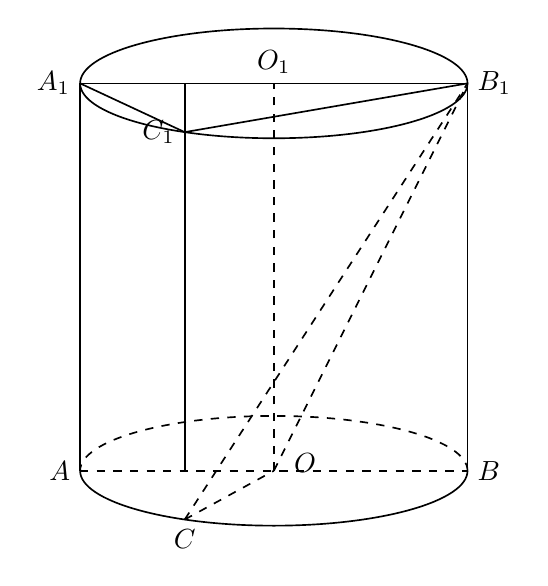
\begin{tikzpicture}[scale=0.82, semithick]
  \def\rx{3}
  \def\ry{0.85}
  \def\H{6}
  \def\cx{-1.38}
  \def\cy{-0.755}

  % 下底：前半（靠观察者）实线，后半虚线
  \draw[dashed] (\rx,0) arc[start angle=0, end angle=180, x radius=\rx, y radius=\ry];
  \draw (-\rx,0) arc[start angle=180, end angle=360, x radius=\rx, y radius=\ry];
  % 下底直径 AB（虚线）与轴 OO1（虚线）
  \draw[dashed] (-\rx,0) -- (\rx,0);
  \draw[dashed] (0,0) -- (0,\H);

  % 上底椭圆（整体可见，实线）
  \draw (0,\H) ellipse[x radius=\rx, y radius=\ry];

  % 三条母线
  \draw (-\rx,0) -- (-\rx,\H);
  \draw (\cx,0) -- (\cx,\H);
  \draw (\rx,0) -- (\rx,\H);

  % 上底：直径 A1B1 与内接三角形 A1B1C1
  \draw (-\rx,\H) -- (\rx,\H);
  \draw (-\rx,\H) -- (\cx,\H+\cy);
  \draw (\cx,\H+\cy) -- (\rx,\H);

  % 虚线：CO、OB1、CB1
  \draw[dashed] (\cx,\cy) -- (0,0);
  \draw[dashed] (0,0) -- (\rx,\H);
  \draw[dashed] (\cx,\cy) -- (\rx,\H);

  \node[left]   at (-\rx,0)      {$A$};
  \node[right]  at (\rx,0)       {$B$};
  \node[below]  at (\cx,\cy)     {$C$};
  \node[left]   at (-\rx,\H)     {$A_1$};
  \node[right]  at (\rx,\H)      {$B_1$};
  \node[left]   at (\cx,\H+\cy)  {$C_1$};
  \node[right]  at (0.16,0.12)   {$O$};
  \node[above]  at (0,\H)        {$O_1$};
\end{tikzpicture}
